\section{Resting atmosphere}
\label{sec:resting}

This two-dimensional test simulates a stably stratified atmosphere in hydrostatic balance.  Since there are no net forces, the analytical solution should remain at rest.  The test specification follows that from \textcite{klemp2011}.  \TODO{again, what is this designed to test?  Klemp says the horiz pressure gradient.  Good says the inversion layer introduces nonlinearity to tax the model even more}

\subsection{Specification}
Following \textcite{weller-shahrokhi2014}, the domain is \SI{20}{\kilo\meter} wide and \SI{20}{\kilo\meter} high, which is narrower than \textcite{klemp2011} in order to reduce simulation time.  The wave-shaped mountain profile is taken from \textcite{schaer2002} where the surface height $h$ is given by
\begin{align}
\surface(x) = \surface_0 \exp \left( - \left( \frac{x}{a} \right)^2 \right) \cos^2 \left( \frac{\pi x}{\lambda} \right)
\end{align}
where $a = \SI{5}{\kilo\meter}$ is the mountain half-width, $h_0 = \SI{1}{\kilo\meter}$ is the maximum mountain height and $\lambda = \SI{4}{\kilo\meter}$ is the wavelength.  For the SLEVE grid, the large-scale component $\surface_1$, described in section~\ref{sec:theory:sleve}, is specified as
\begin{align}
\surface_1(x) = \frac{1}{2} \surface_0 \exp \left( - \left( \frac{x}{a} \right)^2 \right)
\end{align}
and, following \cite{leuenberger2010}, $s_1 = \SI{4}{\kilo\meter}$ is the large scale height, $s_2 = \SI{1}{\kilo\meter}$ is the small scale height, and the optimal exponent value of $n = 1.35$ is used.  Results are compared with the numerical solution with no orography.

The initial thermodynamic conditions have a surface temperature of $\theta_0 = \SI{288}{\kelvin}$ and constant stability with Brunt-V\"ais\"al\"a frequency $N = \SI{0.01}{\per\second}$ everywhere, except for a more stable layer of $N = \SI{0.02}{\per\second}$ between $\SI{2}{\kilo\meter} \leq z \leq \SI{3}{\kilo\meter}$.

\subsection{Diagnostics}
Two metrics were used to measure the model error.  First, maximum vertical velocity is measured at each timestep.  An analytic solution has no vertical velocity $w$ since the atmosphere is at rest.  However, numerical error in calculating the horizontal pressure gradient give rise to spurious vertical velocities which become more severe over steep terrain \autocite{klemp2011}.

Second, energy change $\Delta E$ is measured for each timestep by comparing with the energy in the initial conditions, that is
\begin{align}
	\Delta E(t) &= E(t) - E(t = \SI{0}{\second})
%
	\intertext{where energy is kinetic $E_K$, potential $E_P$, or internal $E_I$, given by \TODOsidenote{check these with Hilary}}
%
	E_K &= \frac{0.25 \sum_{surface} \frac{UV}{\rho}}{\sum V} / \sum_{cells} V \\
	E_P &= - \rho g / \sum_{cells} V \\
	E_I &= \rho \theta \Pi c_v / \sum_{cells} V
\end{align}
An analytic solution would conserve energy such that $\Delta E(t) = 0 \forall t$.  \TODO{why would we expect our model to lose energy?}

\subsection{Discretisation}
The simulation uses the discretisation of the fully-compressible Euler equations described in section~\ref{sec:method:discretisation}.  The domain is discretised on a grid having $40 \times 40$ cells such that $\Delta x = \Delta z = \SI{0.5}{\kilo\meter}$.  All boundary conditions are no slip.  The simulation is integrated forward by 5 hours with a timestep $\Delta t = \SI{100}{\second}$.  Unlike \textcite{klemp2011}, there is no eddy diffusion in our equation set.


\subsection{Results}
Test results for BTF, optimised SLEVE, and SnapCol grids are compared with results on a regular grid with no orography.  On the BTF grid, spurious vertical velocity $w$ reaches $\sim \SI{35}{\centi\meter\per\second}$, which is significantly less than the velocities of $\sim \SI{10}{\meter\per\second}$ found by \textcite{klemp2011} (see figure~\ref{fig:resting:w}, note different vertical scales).  A computational oscillation develops after 4 hours, the cause of which is not yet known.  The optimised SLEVE grid does not significantly reduce $w$ compared to BTF; in fact, an increase is seen at some points during the simulation.

The SnapCol grid results in a significantly smaller maximum vertical velocity of less than \SI{1}{\milli\meter\per\second}.  The smallest error of $\sim \SI{1e-10}{\meter\per\second}$ is found on the regular grid.  This may be due to truncation, but the source of the error has not yet been determined.  Using a timestep of \SI{1.01}{\second}, \textcite{good2013} found the maximum vertical velocity in their cut cell model was \SI{1e-12}{\meter\per\second}, which is better than any result from our experiments.

\TODO{if I want to compare to Zaengl (and also Good), I would need to try the same experiment with 4km high mountain, too}

\begin{figure}
	\captionsetup[subfigure]{position=b}
	\centering
	\subcaptionbox{Model results}[0.58\textwidth]{\input{resting-w-plot}}
	\hfill
	\subcaptionbox{Results from \textcite{klemp2011}}[0.4\textwidth]{\vspace{0.27in}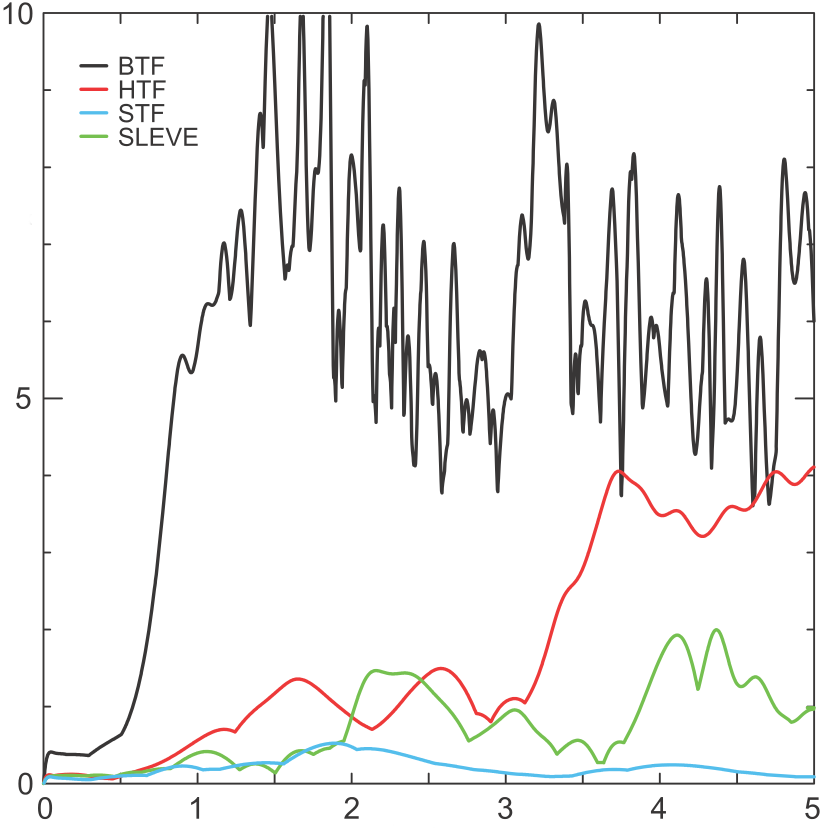
\includegraphics[height=2in]{img/klemp-w.png}}
	\caption{Maximum spurious vertical velocity $w$ in the resting atmosphere test}
	\label{fig:resting:w}
\end{figure}
% Compare vertical velocities with Klemp 2011 (and Weller 2014...)
% Compare energy change
% mention computational thingy >5hrs on BTF?
% could compare theta field (as done by Klemp)


\hrule

Compared meshes, and dp/dx versus H operator.

\begin{itemize}
\item Energy change compared (see Figure~\ref{fig:rest:energy-tf}, \ref{fig:rest:energy-cut-cell})
\item H operator always outperforms dp/dx
\item All cut-cell style meshes outperform TF meshes in this test in terms of $w$ and energy change
\end{itemize}
Some issues were found:
\begin{itemize}
\item noOrography should have zero $w$, but actually has \SI{1e-10}{\meter\per\second}.  Hilary says this is due to loss of precision when reading initial fields (should be in discrete hydrostatic balance).
\item Computational oscillation in BTF H operator after about 4 hours (Figure~\ref{fig:rest:energy-tf})
\end{itemize}

\begin{figure}
BTF H
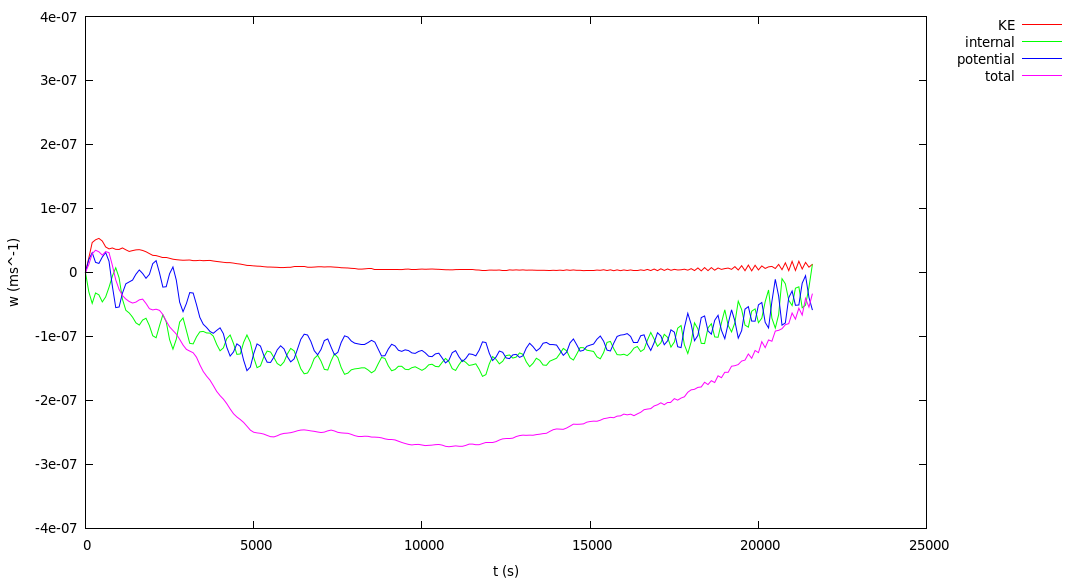
\includegraphics[width=\textwidth]{interim-results/restingBtfHEnergy.png}
SLEVE
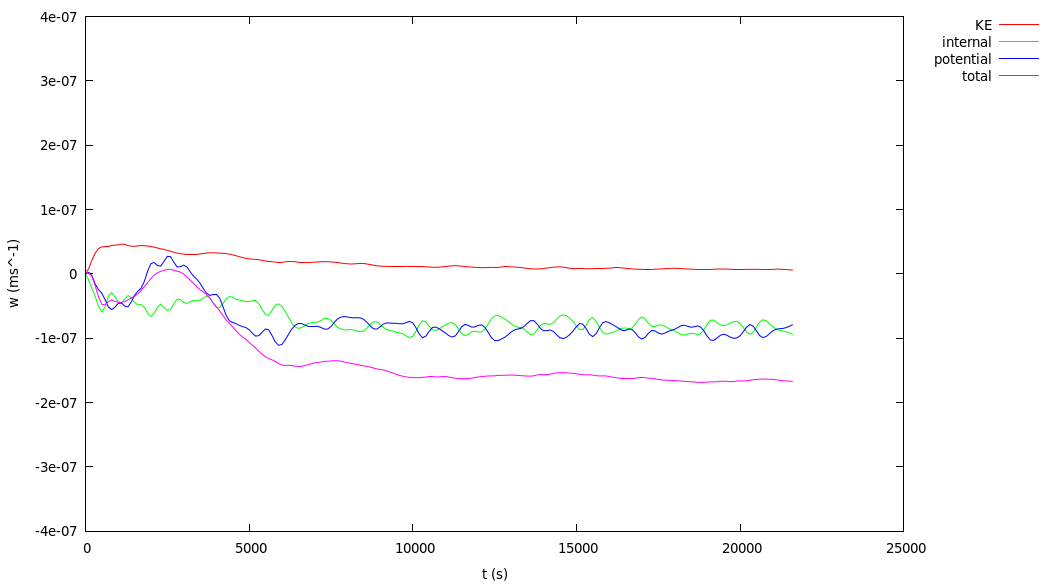
\includegraphics[width=\textwidth]{interim-results/restingSleveEnergy.png}
\caption{Energy changes (TF)}
\label{fig:rest:energy-tf}
\end{figure}

\begin{figure}
SnapCol
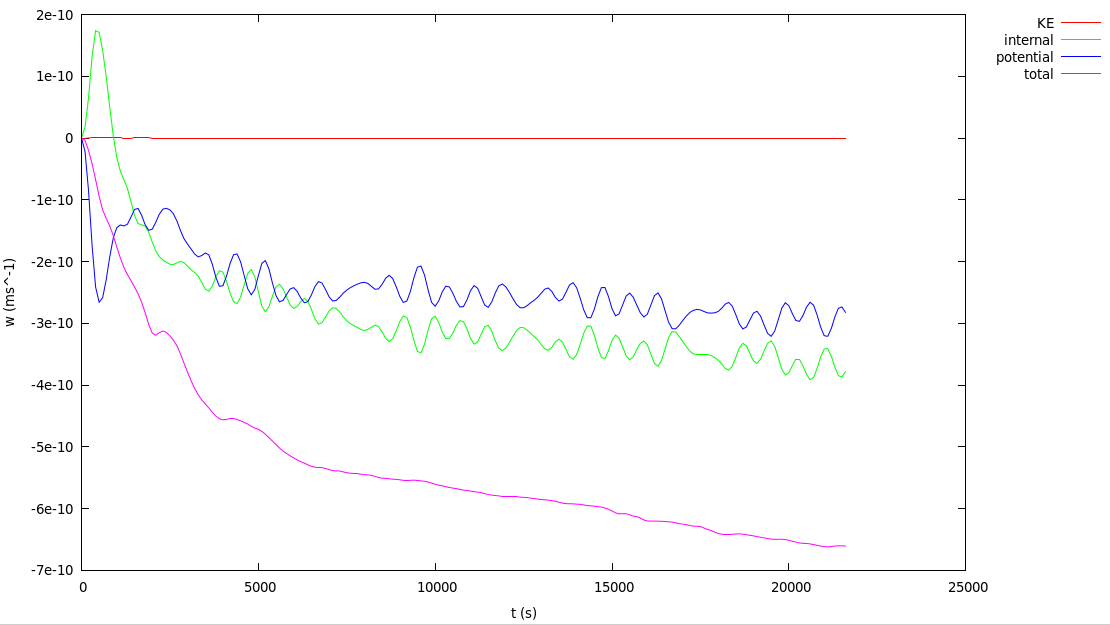
\includegraphics[width=\textwidth]{interim-results/restingSnapColEnergy.png}
\caption{Energy changes (cut-cell style)}
\label{fig:rest:energy-cut-cell}
\end{figure}
